\section*{Simulator}
    A python simulation was realized using VIBES in order to test the behavior of the system. A class \textit{Tank} has been created to instantiate a vehicle with its sled. Then the script integrates the evolution equation using Euler's method in order to obtain the state of the system $x$ according to the $u$ inputs. We could see that the behavior of the system seems correct and the model is faithful to reality. Moreover, the GNSS sensor and an accelerometer are simulated in order to enclose the real position in a box.

    \begin{figure}[!htb]
        \centering
        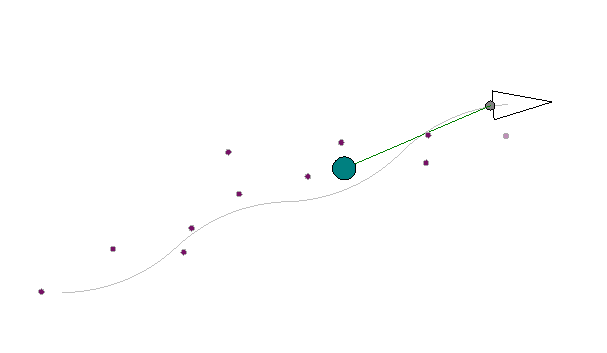
\includegraphics[width=0.35\textwidth]{imgs/simulator.png}
        \caption{\label{fig:simulation} Simulation of the system}
    \end{figure}